%\section{Analysis}

%Explain this figure


\begin{figure*}[th]
\centering
\begin{subfigure}{\textwidth}
  \centering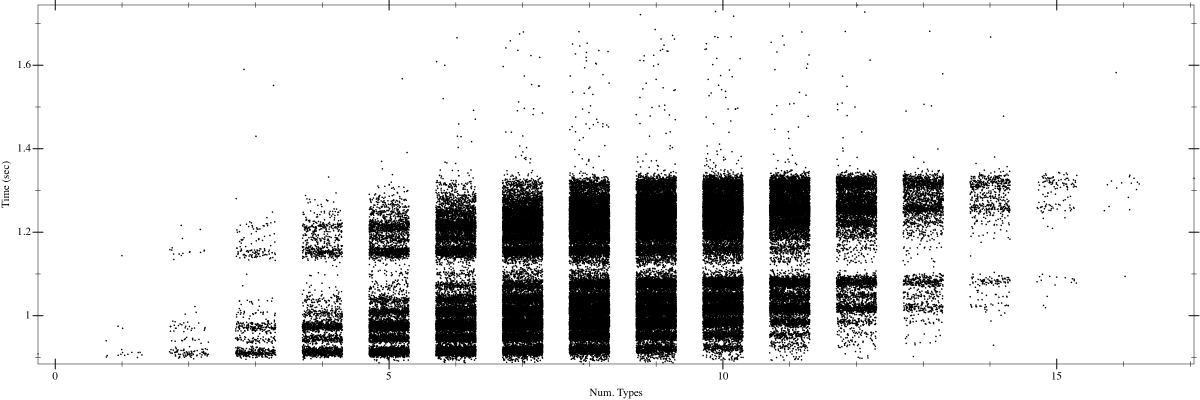
\includegraphics[width=\textwidth]{figures/FSM.png}
  \caption*{Sample FSM - 5 Modules}
\end{subfigure}

\begin{subfigure}{\textwidth}
  \centering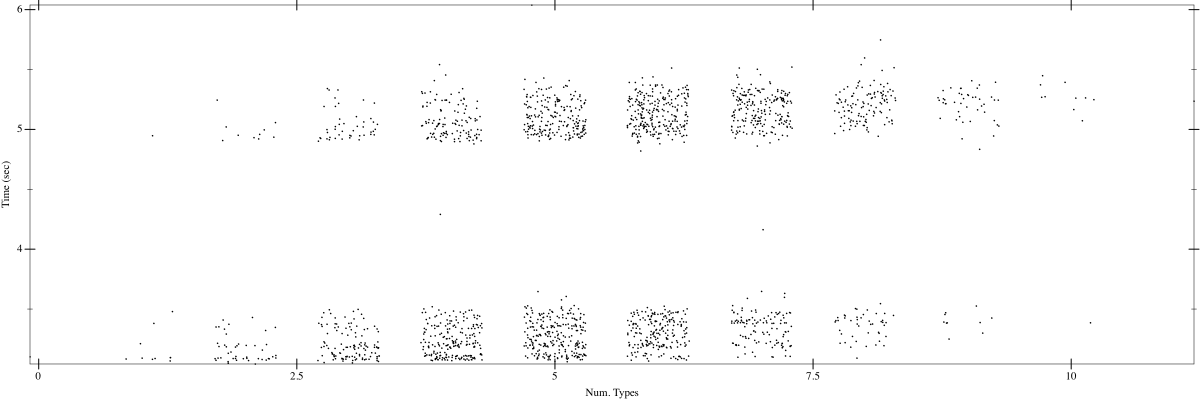
\includegraphics[width=\textwidth]{figures/Espionage.png}
  \caption*{Espionage - 2 Modules}
\end{subfigure}

% Union find causes gap (upper half is when union-find.find is typed
% Lower half is when union-find is untyped.

\begin{subfigure}{\textwidth}
  \centering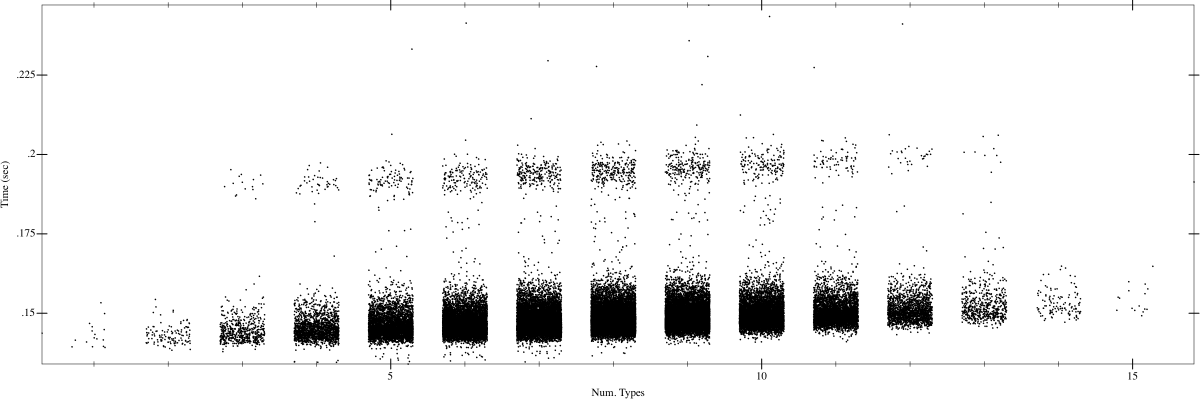
\includegraphics[width=\textwidth]{figures/Evolution.png}
  \caption*{Evolution - 3 Modules}
 \end{subfigure}
\caption{scatterplots}
\label{fig:scatterplots1}
\end{figure*}

\begin{figure*}[t]
  \begin{subfigure}{\textwidth}
    \centering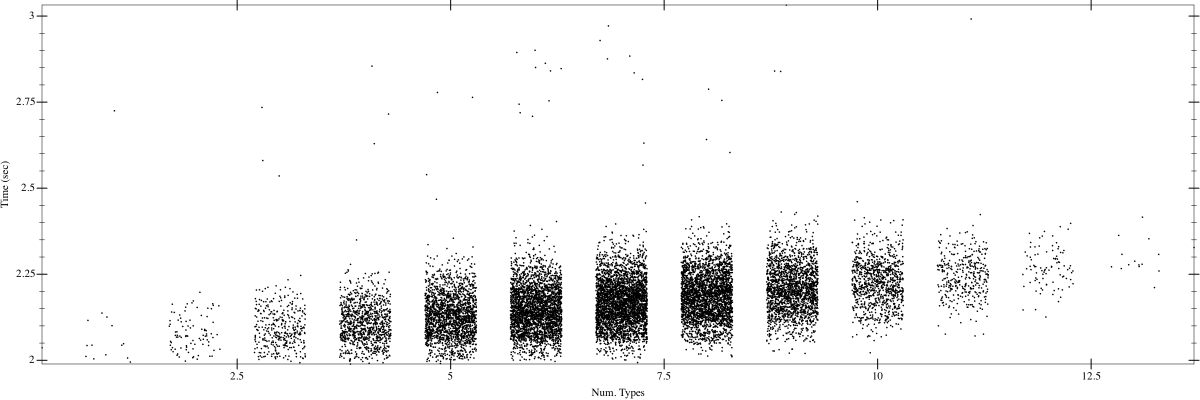
\includegraphics[width=\textwidth]{figures/Take5.png}
  \caption*{Take5 - 3 Modules}
\end{subfigure}

\begin{subfigure}{\textwidth}
  \centering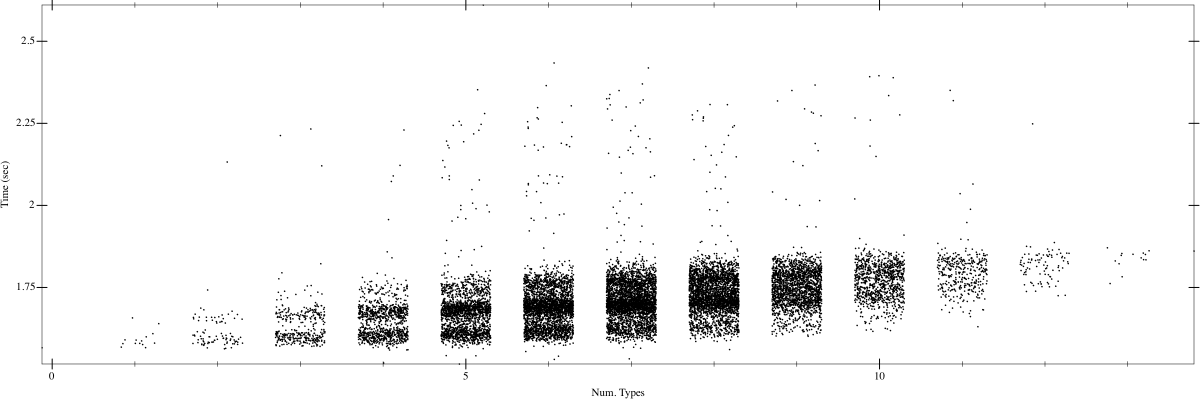
\includegraphics[width=\textwidth]{figures/slowSHA.png}
  \caption*{slow SHA - 4 Modules}
\end{subfigure}

\caption{scatterplots}
\label{fig:scatterplots}
\end{figure*}
Hi~\ref{fig:scatterplots2}

